\documentclass[letterpaper, 12pt]{article}
\usepackage{graphicx}
\usepackage{titling}
\usepackage{float}
\usepackage{csvsimple}
\usepackage{fullpage}

\title{Template}
\date{November 7, 2019}
\author{Faris Hijazi\\
        Phys 4B 1:00-3:50\\}
\begin{document}
\begin{titlingpage}
    \maketitle
    \begin{abstract}
        abstract here
    \end{abstract}
\end{titlingpage}


\section*{Introduction} 

\section*{Equipment}

\begin{itemize}
    \item item 1
    \item item 2
\end{itemize}

\begin{figure}[H]
    \centering
%    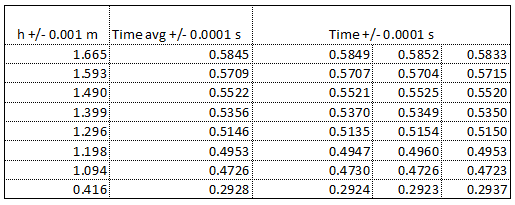
\includegraphics[width=\textwidth]{table}
    \caption{example}
    \label{fig:example}
\end{figure}

\section*{Theory}

\begin{table}[H]
\begin{tabular}{|l|l|}
\hline
\textbf{Variable}   & \textbf{Definition}                                            \\
    \hline
    V                       & Potential Difference                                   \\
    \hline
    \(V_x\)                 & Potential Difference at the unknown resistor           \\
    \hline
    \(V_2 - V_4\)           & potential difference at known resistors                \\
    \hline
    \(R_x\)                 & resistance of unknown resistor                         \\
    \hline
    \(R_x - R_4\)           & resistance of known resistors                          \\
    \hline
    \(L_3, L_4\)            & length of wire split at point of no Galvanometer reading \\
    \hline
    A                       & Amps                                                   \\
    \hline
    \(A\)                   & Area of wire                                           \\
    \hline
    \(\rho\)                & resistivity                                            \\
    \hline                                       
\end{tabular}
\end{table}

\begin{center}
                    eqns go here
\end{center}

\section*{Procedure}

\section*{Analysis}

\subsection*{Data}

\section*{Conclusion}

\end{document}
